\documentclass[a4paper]{ctexart}
\usepackage{xeCJK}
\usepackage{setspace}
\usepackage{graphicx,wrapfig}
\usepackage{fontspec,xunicode,xltxtra}
\usepackage{fancyhdr,titlesec,titletoc}
\usepackage[titletoc]{appendix}
\usepackage[top=29mm,bottom=29mm,left=31.8mm,right=31.8mm]{geometry}
\usepackage{enumerate,enumitem}
\usepackage{caption}
\usepackage{amsmath,amssymb,bm,array}
\usepackage{cite}
\usepackage{diagbox}
\usepackage{algorithm,algorithmicx,algpseudocode}
\usepackage{multirow}
\usepackage{listings}
\usepackage{color}
\setmainfont{Times New Roman}
\setCJKmainfont[BoldFont={Songti SC Bold}]{SimSun}
\setCJKfamilyfont{heiti}{SimHei}
\renewcommand{\heiti}{\CJKfamily{heiti}\fontspec{Times New Roman}}

\newcommand{\mycaptionfont}{\heiti\zihao{5}}
\captionsetup[figure]{name={\mycaptionfont 图},labelsep=period}
\captionsetup[table]{name={\mycaptionfont 表},labelsep=period}
\floatname{algorithm}{\mycaptionfont 算法}
\captionsetup[algorithm]{labelsep=period}
\renewcommand{\captionfont}{\mycaptionfont}
\renewcommand{\captionlabelfont}{\mycaptionfont}

\ctexset {
	section = {
		number = \arabic{section},
		format = \zihao{4}\bfseries,
	},
	subsection = {
		number = \arabic{section}.\arabic{subsection},
		format = \zihao{-4}\bfseries,
	},
	subsubsection = {
		number = \arabic{section}.\arabic{subsection}.\arabic{subsubsection},
		format = \zihao{-4}\bfseries,
	}
}
\setlist[enumerate]{itemindent=2em,listparindent=2em,leftmargin=1em,label=\arabic*、}

\setlength\parskip{.5\baselineskip}
\fancypagestyle{plain}{\pagestyle{fancy}}%改变章节首页页眉
\pagestyle{fancy}
\lhead{\kaishu~硬件综合课程设计报告~}
\rhead{\kaishu~1030616134~尹达恒~}
\cfoot{\thepage}

\definecolor{codegreen}{rgb}{0,0.6,0}
\definecolor{codegray}{rgb}{0.5,0.5,0.5}
\definecolor{codepurple}{rgb}{0.58,0,0.82}
\definecolor{backcolour}{rgb}{0.95,0.95,0.92}

\titlecontents{section}[0em]{\vspace{0.01\baselineskip}\songti\zihao{-4}}{\thecontentslabel\ }{}
{\hspace{.5em}\titlerule*[4pt]{$\cdot$}\contentspage}
\titlecontents{subsection}[2em]{\vspace{0.01\baselineskip}\songti\zihao{-4}}{\thecontentslabel\ }{}
{\hspace{.5em}\titlerule*[4pt]{$\cdot$}\contentspage}
\setcounter{tocdepth}{2}

\begin{document}

\lstdefinelanguage{VHDL}{
	morekeywords=[1]{
			ACCESS,ATTRIBUTE,BEGIN,BODY,BUS,BLOCK,BUFFER,CONSTANT,CASE,COMPONENT,CONFIGURATION,DOWNTO,ELSE,ELSIF,END,ENTITY,EXIT,FUNCTION,FOR,FILE,GENERIC,GENERATE,GUARDED,GROUP,IF,IN,INOUT,IS,INERTIAL,IMPURE,LIBRARY,LOOP,LABEL,LITERAL,LINKAGE,MAP,MOD,NOT,NOR,NAND,NULL,NEXT,NEW,OUT,OF,OR,OTHERS,ON,OPEN,PROCESS,PORT,PACKAGE,PURE,PROCEDURE,POSTPONED,RANGE,REM,ROL,ROR,REPORT,RECORD,RETURN,REGISTER,REJECT,SIGNAL,SUBTYPE,SLL,SRL,SLA,SRA,SEVERITY,SELECT,THEN,TYPE,TRANSPORT,TO,USE,UNITS,UNTIL,VARIABLE,WHEN,WAIT,WHILE,XOR,XNOR,DISCONNECT,ELIF,WITH},% Arnaud Tisserand
	sensitive=f,% 1998 Gaurav Aggarwal
	morestring=[d]{"},%
	morekeywords=[2]{
			std_logic_vector,std_logic,std_logic_1164,numeric_std,numeric_signed,numeric_unsigned,numeric_bit,math_real,math_complex,
			unsigned,integer,
			rising_edge,to_integer,resize
		},
	morecomment=[l]--
}

\lstset{
	language={VHDL},
	numbers=left,numberstyle=\tiny,
	basicstyle=\small\ttfamily,
	stringstyle=\color{codepurple},
	keywordstyle=\color{blue}\bfseries,
	commentstyle=\color{codegreen},
	rulesepcolor=\color{codegray},
	tabsize=2
}

\tableofcontents
\newpage

\begin{center}
	{\zihao{-3}\textbf{简单CPU硬件结构和微指令设计}}

	{\zihao{-4}尹达恒}\\[-1mm]

	{\zihao{5}(江南大学物联网工程学院,江苏\quad 无锡)}
\end{center}
\begin{spacing}{1.3}
	\songti\zihao{-4}
	\section{设计要求}
	\begin{itemize}
		\item 设计一个由微指令控制的简单加法CPU,使其能从输入寄存器中先后读入两个数进行相加,并将结果存入输出寄存器;
		\item 设计一个由微指令控制的循环加法CPU,使其能从输入寄存器中先后读入多个数进行相加,并将结果存入输出寄存器。
	\end{itemize}
	\section{总体设计}
	\subsection{硬件结构}
	根据设计要求,简单CPU硬件结构将包含以下元件:
	\begin{itemize}
		\item 一个控制器;
		\item 一个数据总线;
		\item 一个算术逻辑单元;
		\item 四个寄存器(两个数据寄存器、一个输入寄存器、一个输出寄存器)。
	\end{itemize}

	总体设计图如图\ref{fig:总体结构图}。图中各部分作用如下:
	\begin{itemize}
		\item 输入寄存器:存储将要输入到数据总线中的值;
		\item 数据寄存器1/2:存储将要进行算术逻辑运算的值;
		\item 输出寄存器:存储将要输出的值;
		\item 算术逻辑单元:对数据寄存器1/2中的值进行算术逻辑运算;
		\item 数据总线:负责数据在寄存器之间的转移;
		\item 控制器:对微指令进行译码,控制上述所有部分的动作。
	\end{itemize}
	\begin{figure}[htbp]
		\centering
		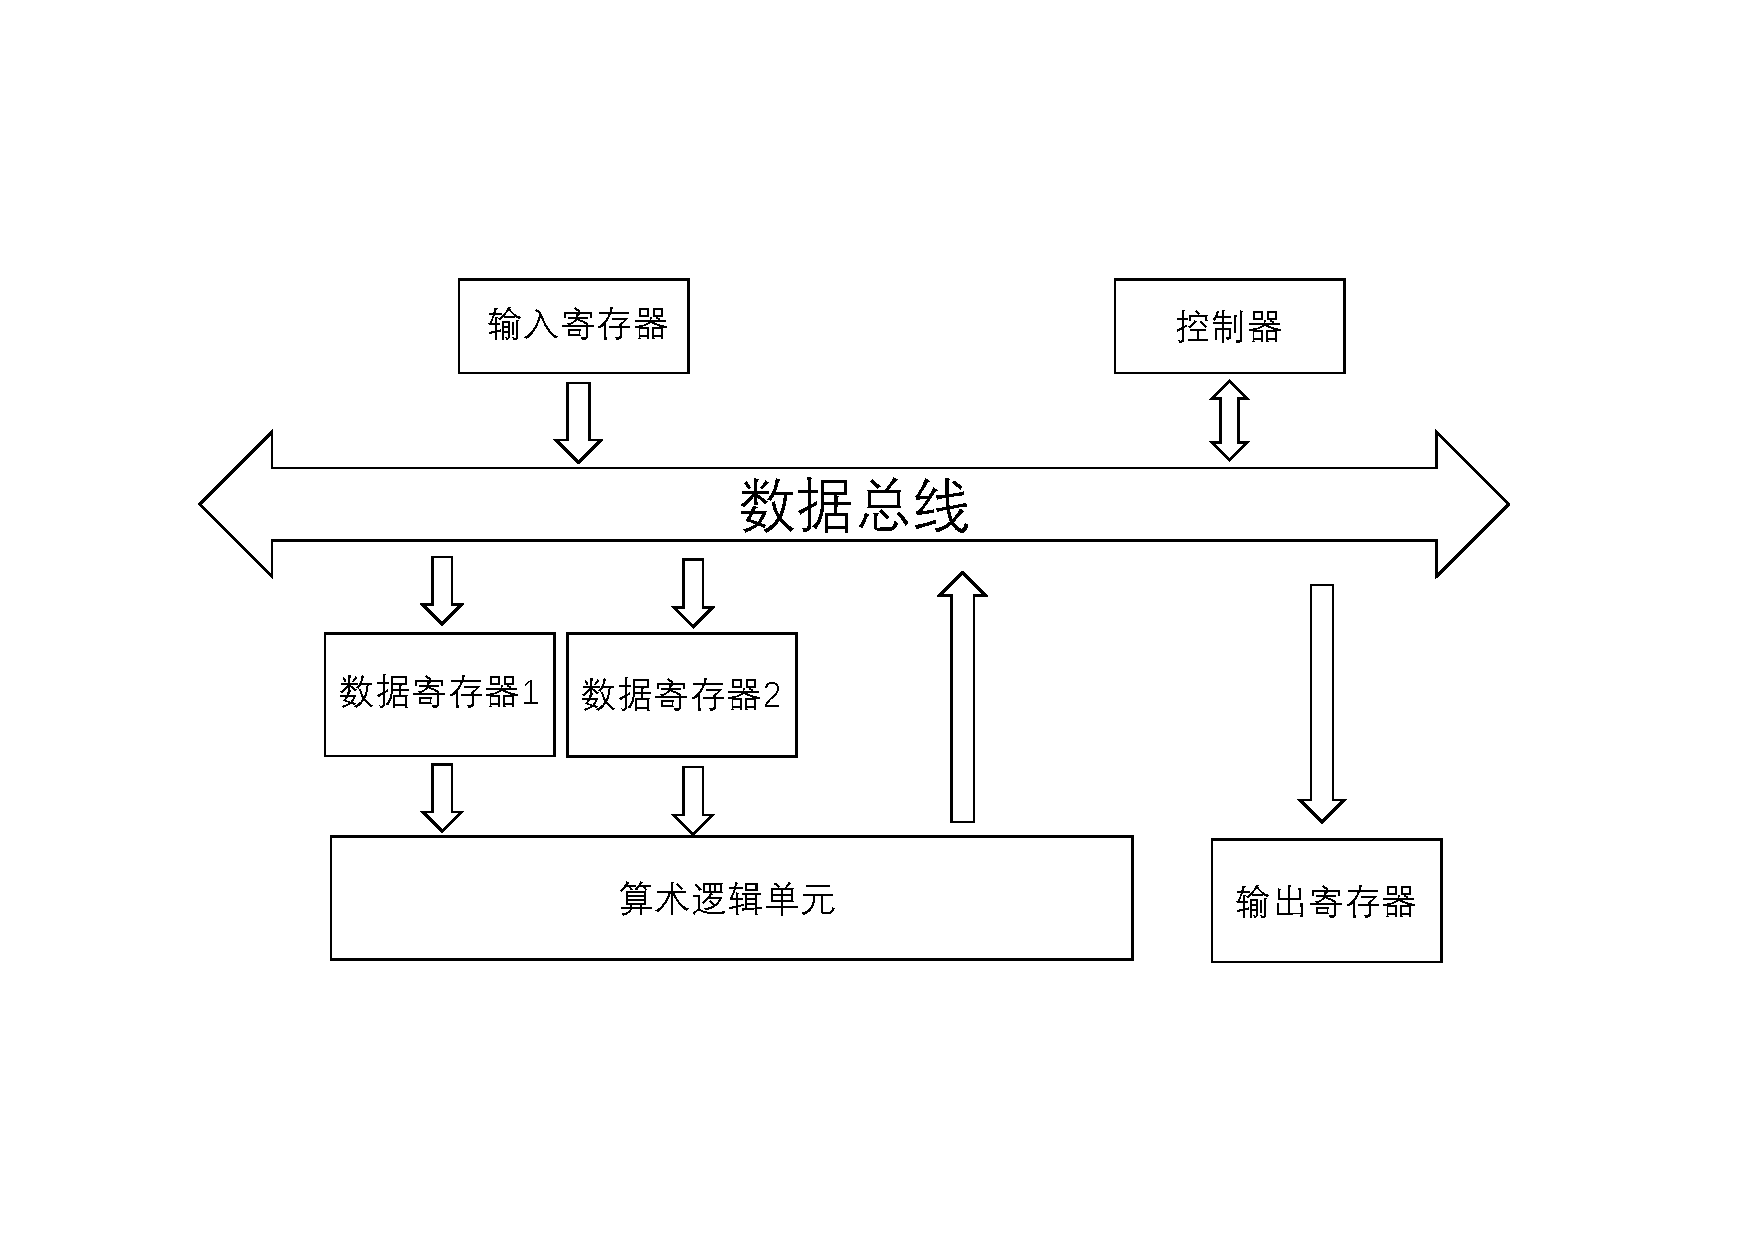
\includegraphics[width=\textwidth]{figure/all.pdf}
		\caption{硬件总体结构}\label{fig:总体结构图}
	\end{figure}

	\subsection{指令结构}
	根据设计要求,简单CPU指令集将至少包含以下功能:
	\begin{itemize}
		\item 将输入寄存器中的值存入数据总线中;
		\item 将数据总线中的值存入数据寄存器1/2或输出寄存器中;
		\item 将算术逻辑单元中的运算结果存入数据总线中。
	\end{itemize}

	且为了能够使用实验板上的开关阵列进行实验,CPU指令集按顺序执行的相邻指令之间必须只能有一位不同。

	\section{硬件结构设计}

	\subsection{各元件选型及特性}\label{各元件选型及特性}

	\subsubsection{输入寄存器元件reg\_74244}
	输入寄存器使用ISE自带的寄存器元件reg\_74244,其元件示意图如图\ref{fig:reg_74244}。该元件在输出使能端口oen为低电平时使输出端口Qout(7:0)的8位电平状态与输入端口Din(7:0)相同。
	\begin{figure}[htbp]
		\centering
		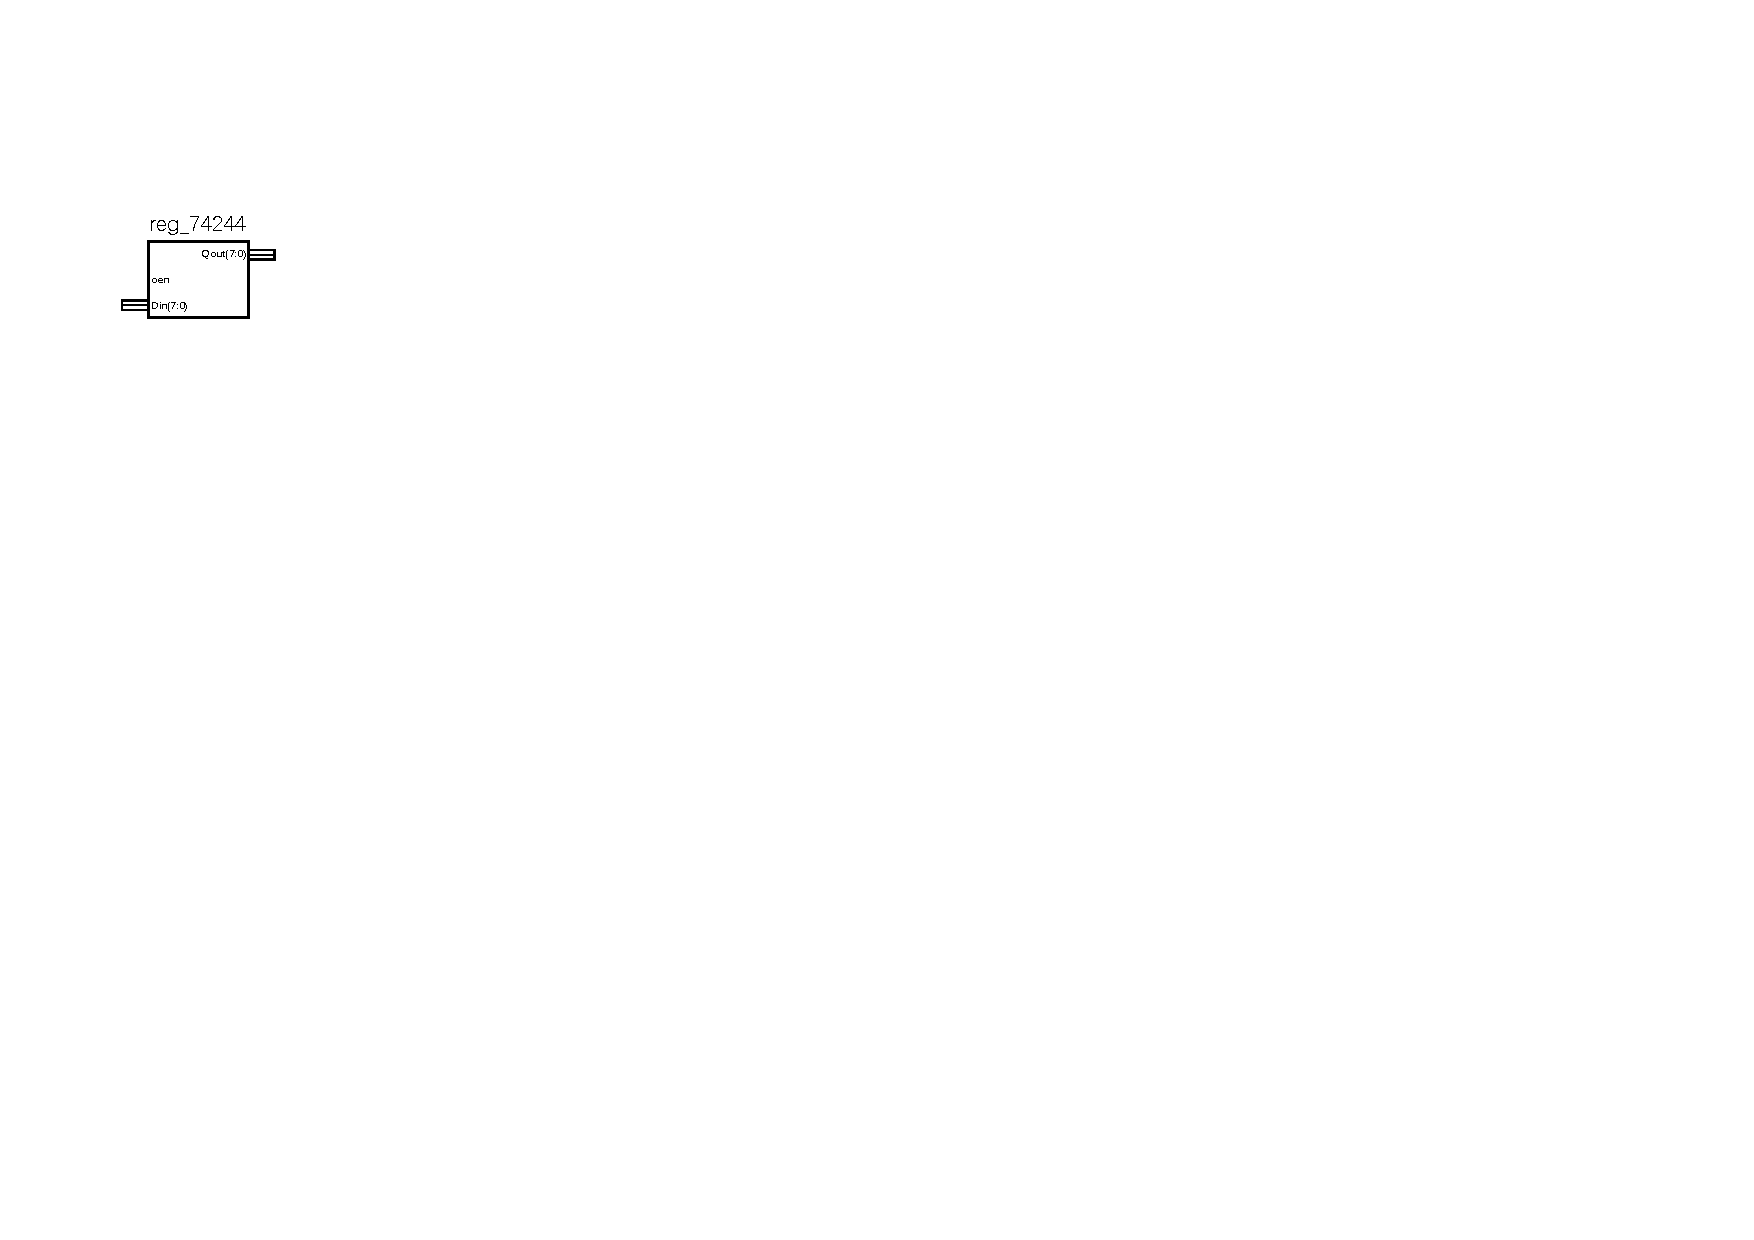
\includegraphics[width=0.47\textwidth]{figure/reg_74244.pdf}
		\caption{reg\_74244元件示意图}\label{fig:reg_74244}
	\end{figure}

	\subsubsection{数据寄存器1/2和输出寄存器元件reg\_74373}
	数据寄存器和输出寄存器使用ISE自带的寄存器元件reg\_74373,其元件示意图如图\ref{fig:reg_74373}。该元件在时钟端口clk输入一个时钟脉冲时有以下动作:
	\begin{itemize}
		\item 若输出使能端口oen\_n为低电平,则使输出端口Qout(7:0)的8位电平状态与内部寄存值相同;
		\item 若输入使能端口gwe为高电平,则将输入端口Din(7:0)的值写入内部寄存器。
	\end{itemize}
	\begin{figure}[htbp]
		\centering
		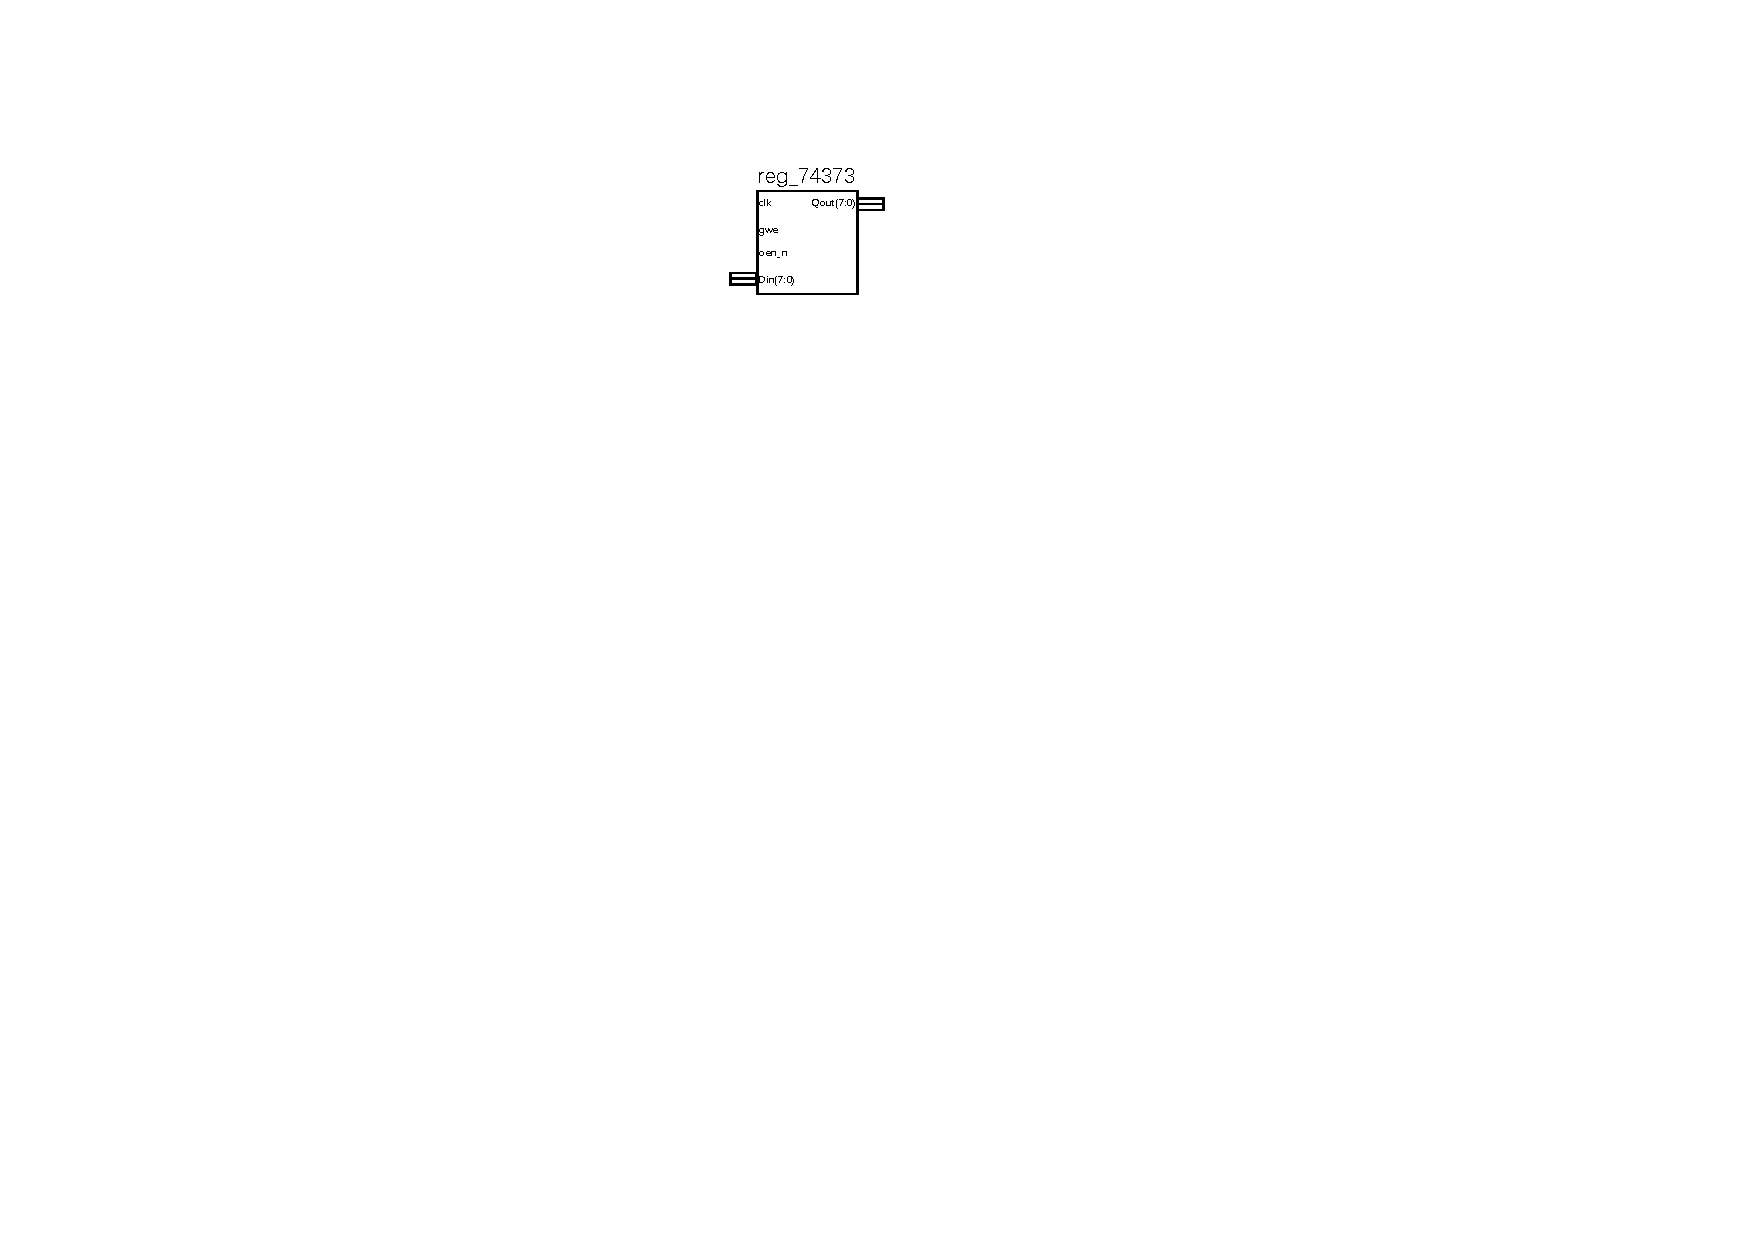
\includegraphics[width=0.47\textwidth]{figure/reg_74373.pdf}
		\caption{reg\_74373元件示意图}\label{fig:reg_74373}
	\end{figure}

	\subsubsection{算术逻辑单元alu\_74181}
	由于ISE自带的算术逻辑单元alu\_74181为四位运算器,无法满足本设计方案中八位运算器的需求,因此需要进行修改,修改后的VHDL代码如附录\ref{alu_74181程序}所示,其元件示意图如图\ref{fig:alu_74181}。该元件的输入端口C\_n、A(7:0)、B(7:0)和输出端口C\_n\_plus4、F(7:0)的关系受输入端口S(4:0)的值控制。其中当S(4:0)端口为0110时,F=C\_n+A+B。

	\begin{figure}[htbp]
		\centering
		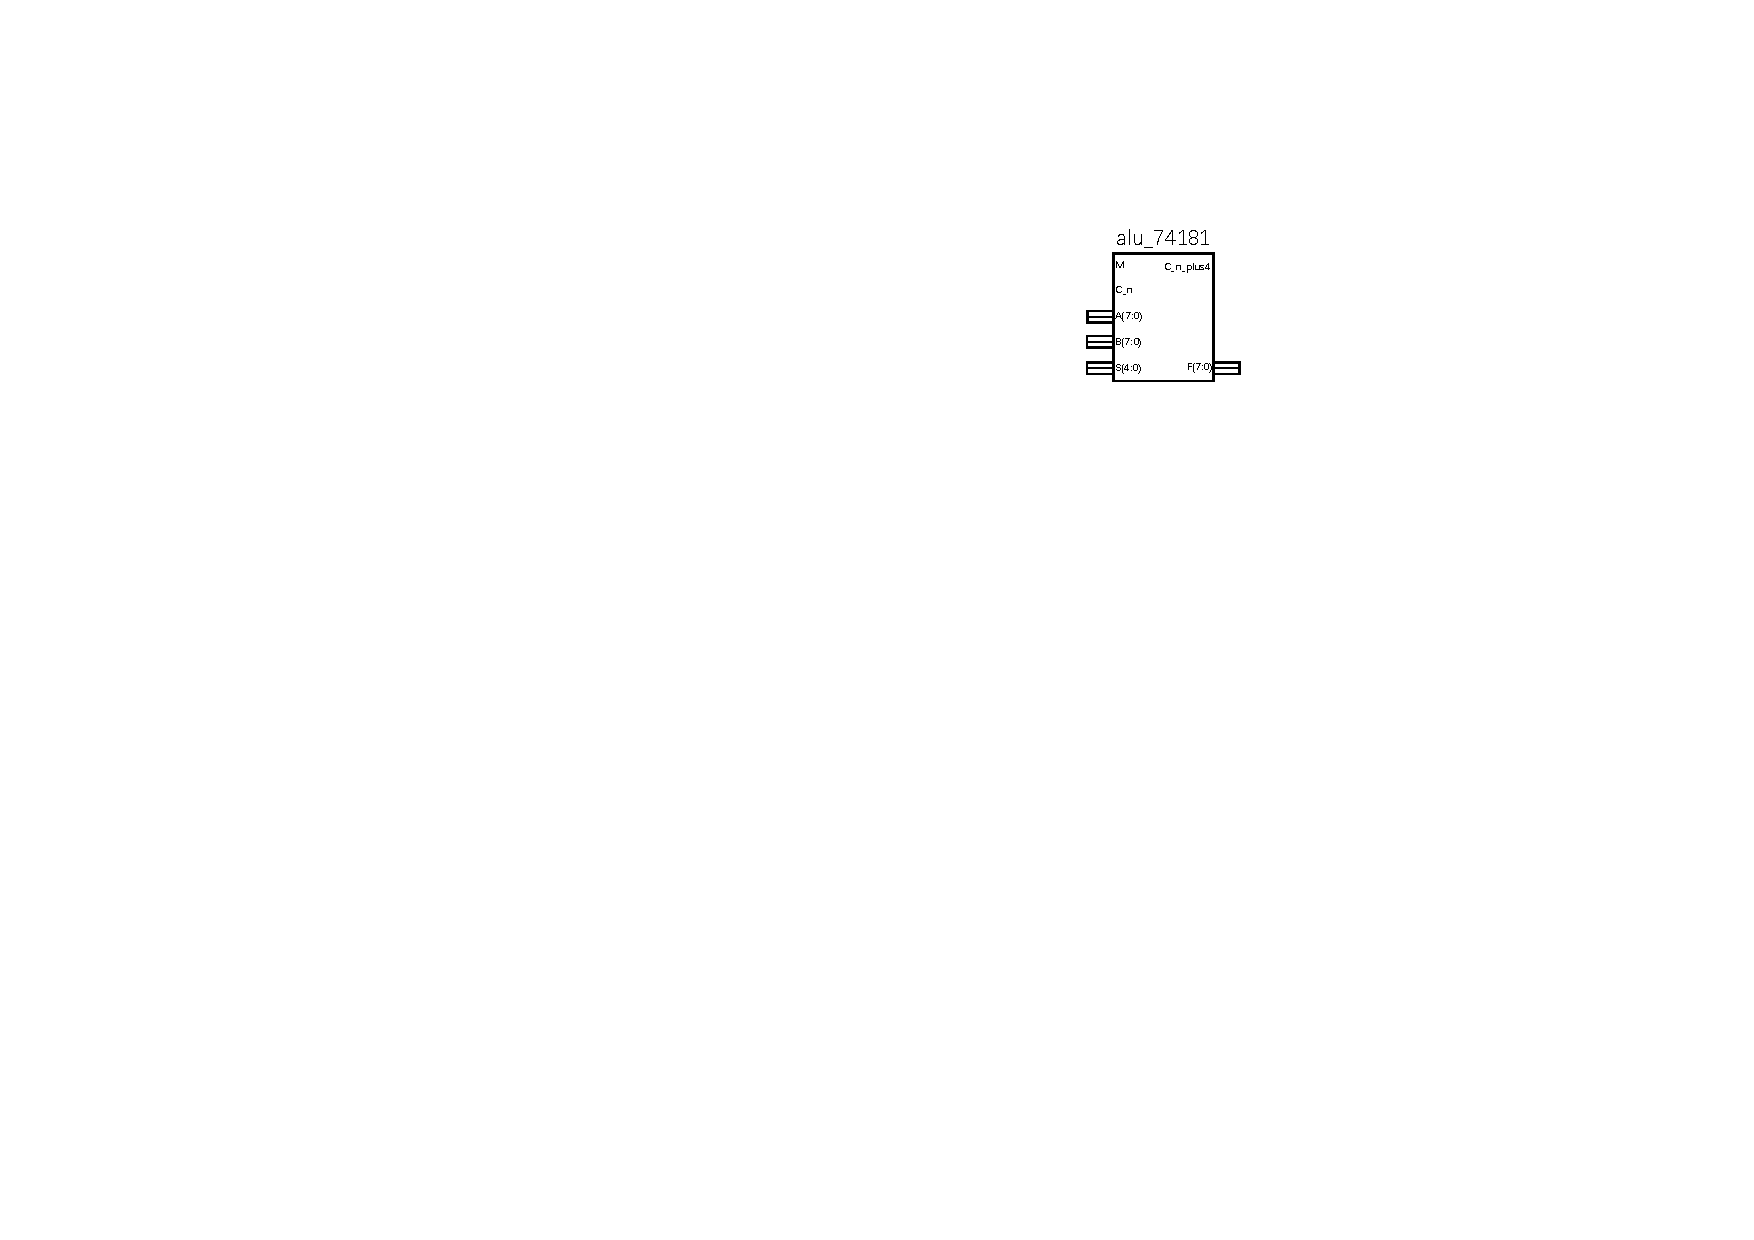
\includegraphics[width=0.47\textwidth]{figure/alu_74181.pdf}
		\caption{alu\_74181元件示意图}\label{fig:alu_74181}
	\end{figure}

	\subsubsection{数据总线data\_bus}
	数据总线使用ISE自带的数据总线元件data\_bus,其元件示意图如图\ref{fig:data_bus}所示。该元件在时钟端口clk输入一个时钟脉冲时有以下动作:
	\begin{itemize}
		\item 若端口we1为高电平,则将端口data\_in1(7:0)的值写入内部寄存器;
		\item 若端口we1为低电平且端口we2为高电平,则将端口data\_in2(7:0)的值写入内部寄存器;
		\item 若端口we1、we2为低电平且端口we3为高电平,则将端口data\_in3(7:0)的值写入内部寄存器;
		\item 若端口we1、we2、we3为低电平且端口we4为高电平,则将端口data\_in4(7:0)的值写入内部寄存器;
		\item 若端口we1、we2、we3、we4为低电平且端口we\_io1为高电平,则将端口data\_io1(7:0)的值写入内部寄存器;
		\item 若端口we1、we2、we3、we4、we\_io1为低电平且端口we\_io2为高电平,则将端口data\_io2(7:0)的值写入内部寄存器;
		\item 使四个八位输出端口data\_out1/2/3/4(7:0)值等于data\_bus内部寄存器的值,若端口we1、we2、we3、we4、we\_io1、we\_io2均为低电平,则使输出端口data\_io1/2(7:0)的值等于内部寄存器的值。
	\end{itemize}

	\begin{figure}[htbp]
		\centering
		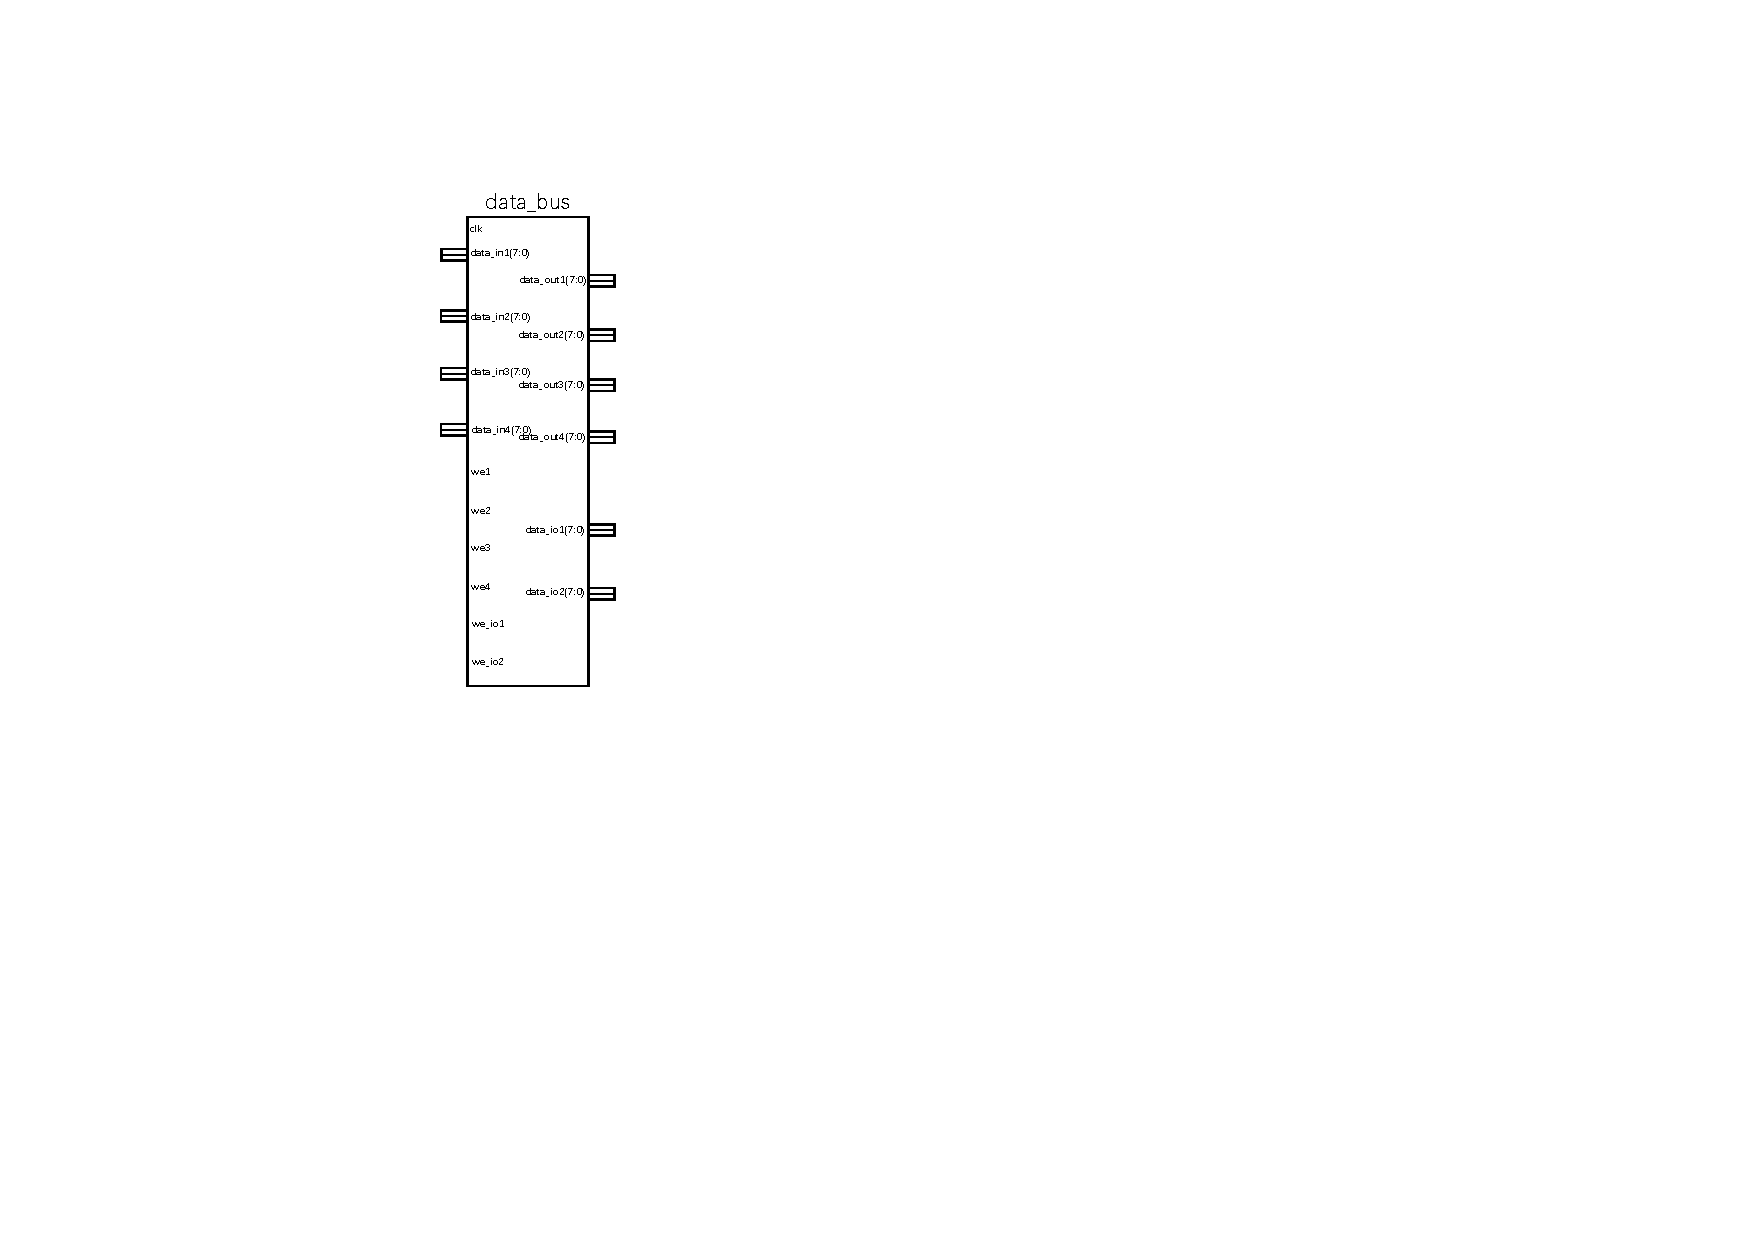
\includegraphics[width=0.47\textwidth]{figure/data_bus.pdf}
		\caption{data\_bus元件示意图}\label{fig:data_bus}
	\end{figure}
	\newpage

	\subsubsection{控制器romc}
	由于ISE自带的算术逻辑单元romc为二四译码器,无法满足本设计方案的需求,因此需要进行修改,修改后的VHDL代码如附录\ref{简单加法器romc程序}和附录\ref{循环加法器romc程序},其元件符号如图\ref{fig:romc}。romc本质上是一个4-9译码器,输入部分S0/S1/S2/S3为四位微指令,剩下9位输出分别接在各元件上控制元件工作。romc元件控制位如表\ref{tab:控制位表}所示。
	\begin{table}[htbp]
		\setstretch{1.5}
		\centering
		\caption{romc元件控制位表}
		\begin{tabular}{|c|c|c|c|c|c|c|c|c|c|}
			\hline
			输出位 & 8     & 7    & 6     & 5    & 4     & 3    & 2   & 1   & 0   \\
			\hline
			控制位 & OENN3 & GWE3 & OENN2 & GWE2 & OENN1 & GWE1 & WE2 & WE1 & OEN \\
			\hline
		\end{tabular}
		\label{tab:控制位表}
	\end{table}

	\begin{figure}[htbp]
		\centering
		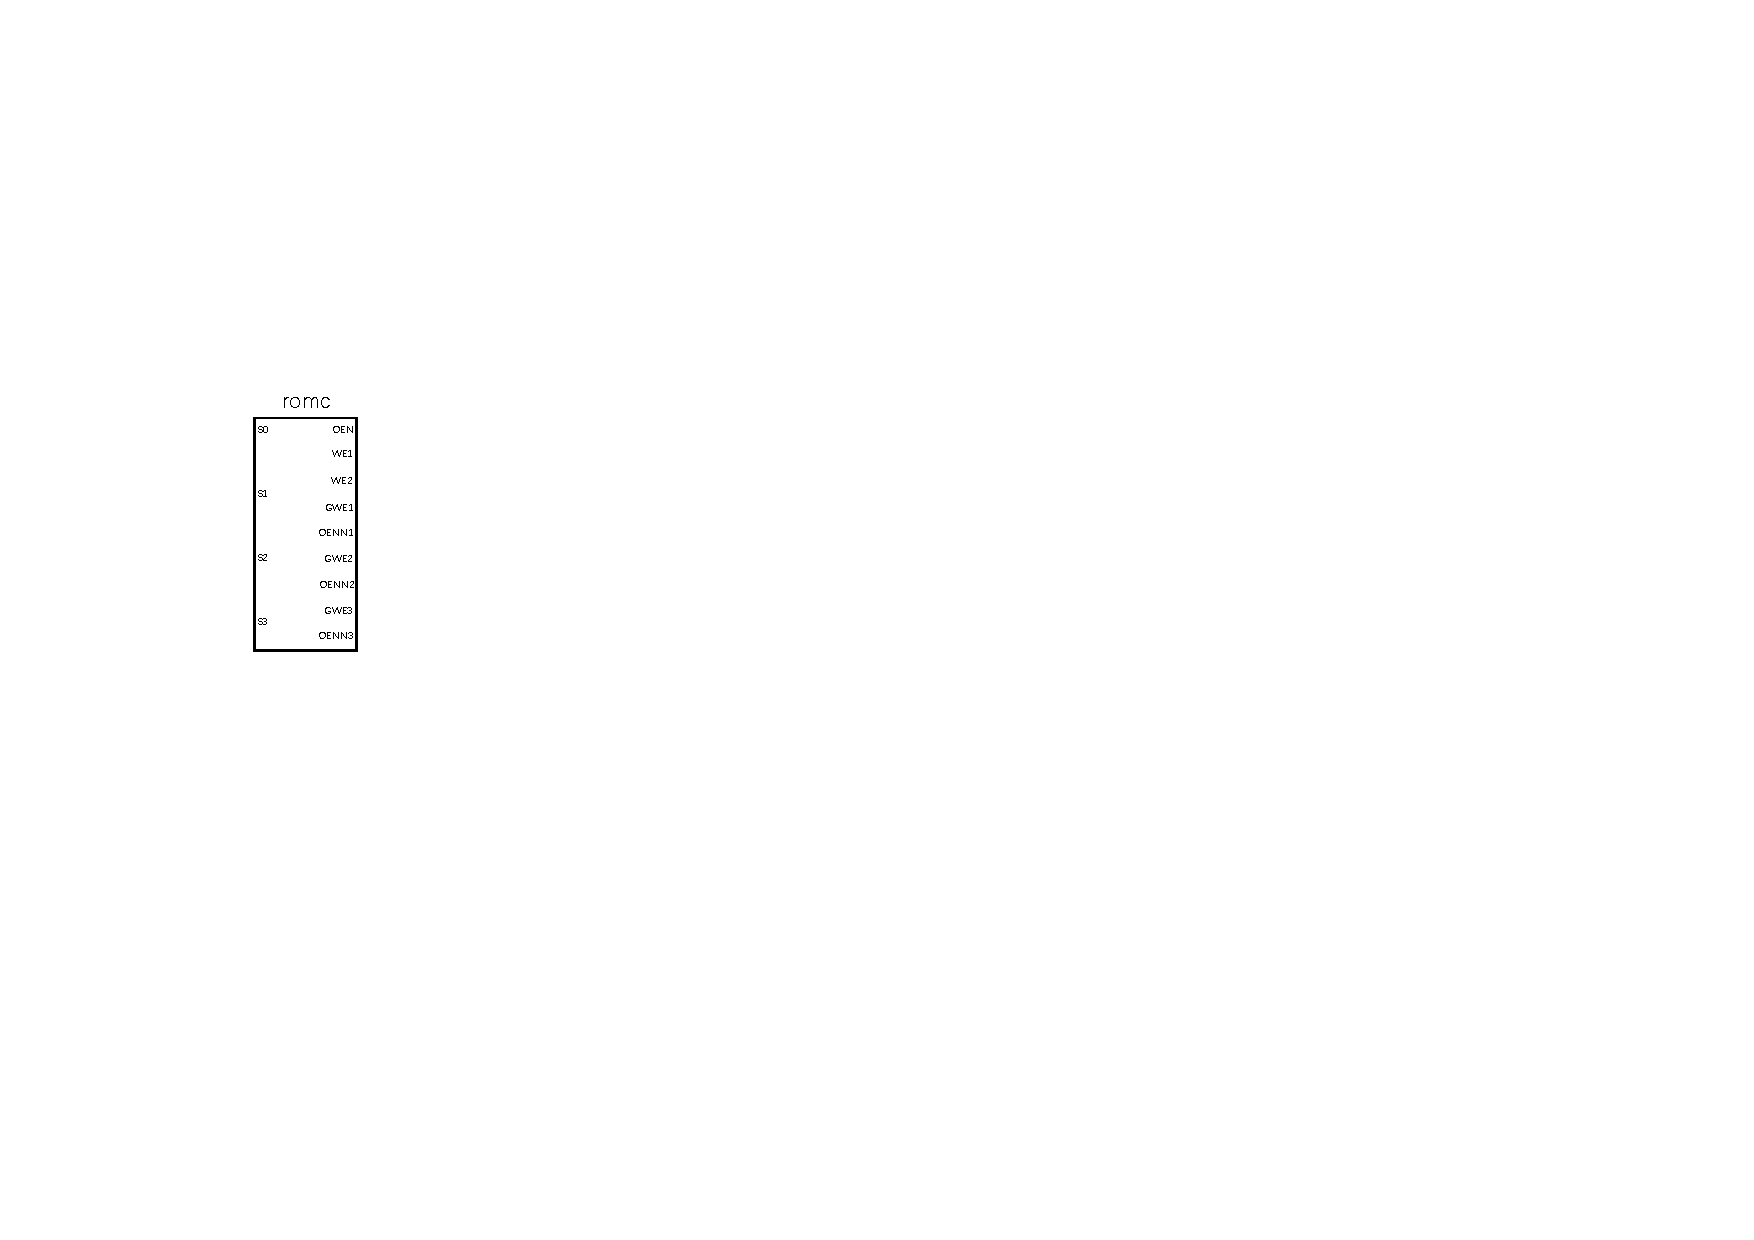
\includegraphics[width=0.3\textwidth]{figure/romc.pdf}
		\caption{romc元件示意图}\label{fig:romc}
	\end{figure}

	\subsection{元件连接}
	\subsubsection{控制器romc的连接方案}\label{控制器romc的连接方案}
	\begin{itemize}
		\item OEN接输入寄存器reg\_74244的使能端oen,控制输入寄存器的使能;
		\item WE1/2分别接数据总线data\_bus的输入使能端we1/2,控制总线读取输入寄存器的值或算术逻辑单元的运算结果;
		\item GWE1/2和OENN1/2分别接数据寄存器1/2的输入使能端gwe和输出使能端oen\_n,控制数据寄存器1/2从数据总线中取数和输出到算术逻辑单元;
		\item GWE3和OENN3分别接输出寄存器的输入使能端gwe和输出使能端oen\_n,控制输出寄存器从数据总线中取数和输出。
	\end{itemize}

	\subsubsection{其他元件的连接方案}
	\begin{itemize}
		\item 输入寄存器reg\_74244:数据输入端口Din接外部数据输入端口DATA\_IN(7:0)、输出端口Qout接数据总线输入端口data\_in1;
		\item 算术逻辑单元alu\_74181:运算控制端口S接外部数据输入端口CTL(3:0)、输入端口A、B分别接数据寄存器1/2的输出端口Qout、输出端口接数据总线输入端口data\_in2;
		\item 输出寄存器reg\_74244:输入端口Din接数据总线输出端口data\_out3、输出端口Qout接数据输出端口DATA\_OUT(7:0);
		\item 数据总线data\_bus:we3、we4、we\_io1、we\_io2接地、data\_out1/2分别接数据寄存器1/2的输入端口Din。
	\end{itemize}

	由上述连接方案得到的元件连接示意图如图\ref{fig:连接示意图}所示。

	\begin{figure}[htbp]
		\centering
		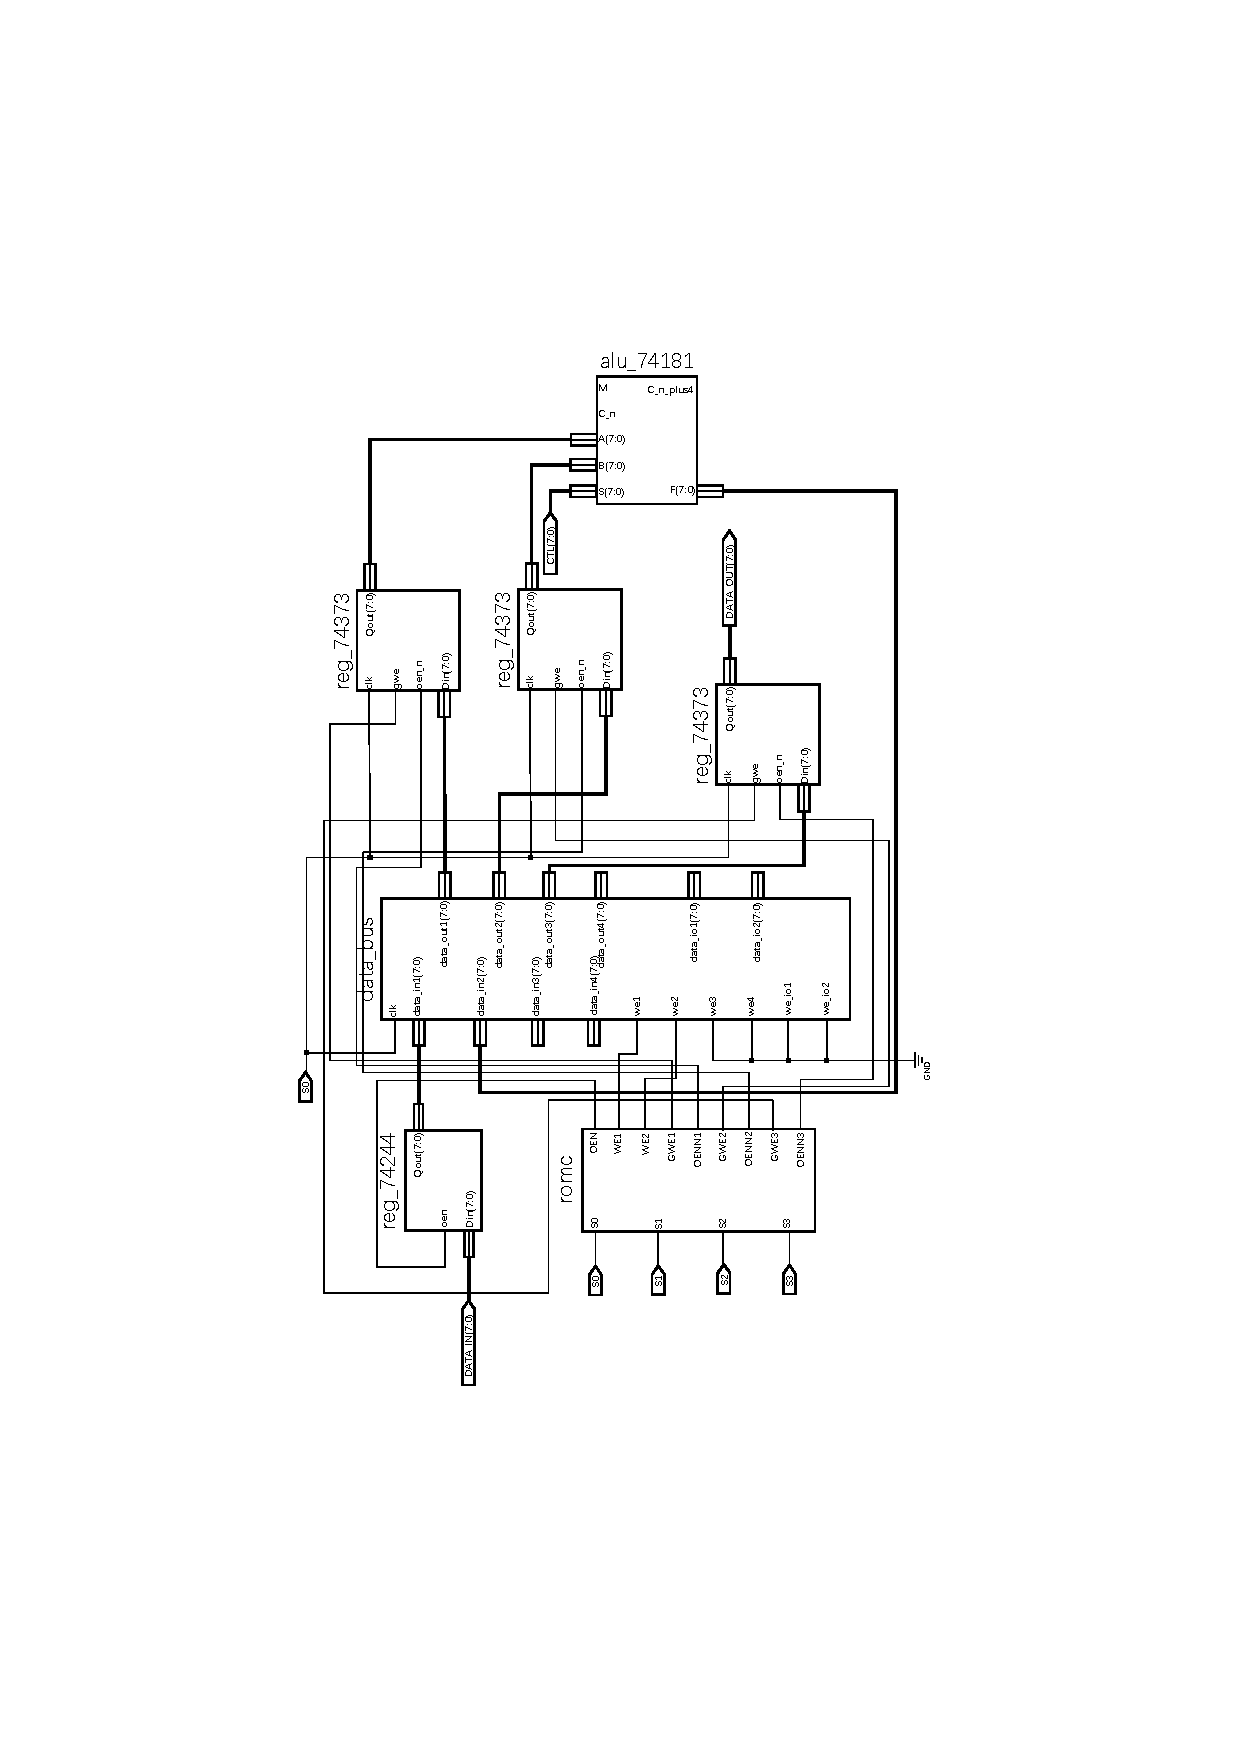
\includegraphics[width=0.95\textwidth]{figure/final.pdf}
		\caption{元件的连接方案示意图}\label{fig:连接示意图}
	\end{figure}

	\subsubsection{外部输入/输出的连接方案}
	\begin{itemize}
		\item 指令输入:romc四个指令输入端口S0/1/2/3分别接Atlys开发板上的开关sw0/1/2/3;
		\item 时钟输入:数据总线data\_bus、数据寄存器1/2和输出寄存器reg\_74373的clk端口接外部时钟输入端口;
		\item 数据输入:外部数据输入端口DATA\_IN(7:0)接EES261的开关SW9$\sim$SW16;
		\item 算术逻辑单元运算控制输入:外部数据输入端口CTL(3:0)在EES261的开关SW5$\sim$SW8;
		\item 数据输出:数据输出端口DATA\_OUT(7:0)接EES261的LED灯LED1$\sim$LED8。
	\end{itemize}

	由上述连接方案编写的外部端口定义文件如附录\ref{外部端口定义}。

	\section{指令结构设计}
	\subsection{简单加法器指令结构设计}\label{简单加法器指令结构}
	由\ref{各元件选型及特性}节所示的元件特性以及\ref{控制器romc的连接方案}节可知,一个加法操作的步骤以及表\ref{tab:控制位表}中对应的romc在一个时钟周期内输出值如下(0表示高电平,1表示低电平,X表示可以为任意值):
	\begin{enumerate}[label=\arabic*、]
		\item 总线从输入寄存器中取出第一个数,romc输出XXXXXXX10;
		\item 总线将取出的数放入数据寄存器1中,romc输出XXXXX1XXX;
		\item 总线从输入寄存器中取出第二个数,romc输出XXXXXXX10;
		\item 总线将取出的数放入数据寄存器2中,romc输出XXX1XXXXX;
		\item 总线从算术逻辑单元中取出结果,romc输出XX0X0X10X;
		\item 总线将取出的数放入输出寄存器中,romc输出X1XXXXXXX。
	\end{enumerate}

	在上述步骤中,某些步骤间的任意值位不重合,可以进行合并,从而使指令更加精简,合并结果如下:
	\begin{enumerate}[label=\arabic*、]
		\item 总线从输入寄存器中取出第一个数并将取出的数放入数据寄存器1中,romc输出XXXXX1X10,经过两个时钟周期完成;
		\item 总线从输入寄存器中取出第二个数并将取出的数放入数据寄存器2中,romc输出XXX1X0X10,经过两个时钟周期完成;
		\item 总线从算术逻辑单元中取出结果并将取出的数放入输出寄存器中输出,romc输出01000010X,经过两个时钟周期完成。
	\end{enumerate}

	指令和romc输出的对应关系不唯一。综合考虑,可以给出romc控制位输出的一个设计方案并为其分配微指令,得到简单加法器的一种指令结构及作用如表\ref{tab:简单加法器指令结构}。以此编写的romc元件定义如附录\ref{简单加法器romc程序}所示。运算器的指令执行步骤是$0000\rightarrow 0001\rightarrow 0011$。
	\begin{table}[htbp]
		\setstretch{1.5}
		\centering
		\caption{简单加法器指令结构}\label{tab:简单加法器指令结构}
		\begin{tabular}{|c|c|c|c|}
			\hline
			步骤   & 微指令 & romc输出 & 作用\\
			\hline
			1 & 0000  & 101011010 & 总线从输入寄存器中取出一个数放入数据寄存器1中\\
			\hline
			2 & 0001  & 101110010 & 总线从输入寄存器中取出一个数放入数据寄存器2中\\
			\hline
			3 & 0011  & 010000100 & 总线从算术逻辑单元中取出结果放入输出寄存器中输出\\
			\hline
		\end{tabular}
	\end{table}


	\subsection{循环加法器指令结构设计}\label{循环加法器指令结构}
	循环加法器指令在简单加法器指令的基础上实现。当算术逻辑单元得出运算结果后,总线从算术逻辑单元中取出结果但不直接放入输出寄存器中,而是再放入数据寄存器中进行下一轮取数-运算的循环。和简单加法器类似,循环加法器指令结构及作用如表\ref{tab:循环加法器指令结构}所示。

	\begin{table}[htbp]
		\setstretch{1.5}
		\centering
		\caption{循环加法器指令结构}\label{tab:循环加法器指令结构}
		\begin{tabular}{|c|c|c|c|}
			\hline
			步骤&微指令&romc输出&作用\\\hline
			1、3&0000&101010010&总线从输入寄存器中取出一个数暂存于总线寄存器\\\hline
			2&0001&101011000&总线将暂存的数放入数据寄存器1中\\\hline
			4&0010&101110000&总线将暂存的数放入数据寄存器2中\\\hline
			5&0011&010000100&总线从算术逻辑单元中取出计算结果暂存并输出\\\hline
			6&0111&101110000&总线将暂存的计算结果放入数据寄存器2中\\\hline
			循环1&1111&101011010&总线从输入寄存器中取出一个数放入数据寄存器1中\\\hline
			循环2&1110&010000100&同0011\\\hline
			循环3&1100&101110000&同0111\\\hline
			循环4&1000&101011010&同1111\\\hline
			循环5&1001&010000100&同0011\\\hline
			循环6&1011&101110000&同0111\\\hline
		\end{tabular}
	\end{table}

	以此编写的romc元件定义如附录\ref{循环加法器romc程序}所示。指令的执行顺序为:$0000\rightarrow 0001\rightarrow 0000\rightarrow 0010\rightarrow 0011\rightarrow 0111$,随后开始指令循环:$1111\rightarrow 1110\rightarrow 1100\rightarrow 1000\rightarrow 1001\rightarrow 1011$。每一轮指令循环都包含两轮“总线从输入寄存器中取出一个数放入数据寄存器1中$\rightarrow$总线将暂存的计算结果放入数据寄存器2中$\rightarrow$总线从算术逻辑单元中取出计算结果暂存并输出”的步骤循环,在每轮步骤循环的第一步输入不同的数,每一轮的运算结果在步骤循环的第二步中输出,即可在保证每一步微指令都只变动一位的情况下实现多个数的循环相加。

\section{运行测试}
\subsection{线路连接}
按图\ref{fig:连接示意图}在ISE软件中进行元件线路连接,结果如图\ref{fig:线路图}。

\begin{figure}[htbp]
	\centering
	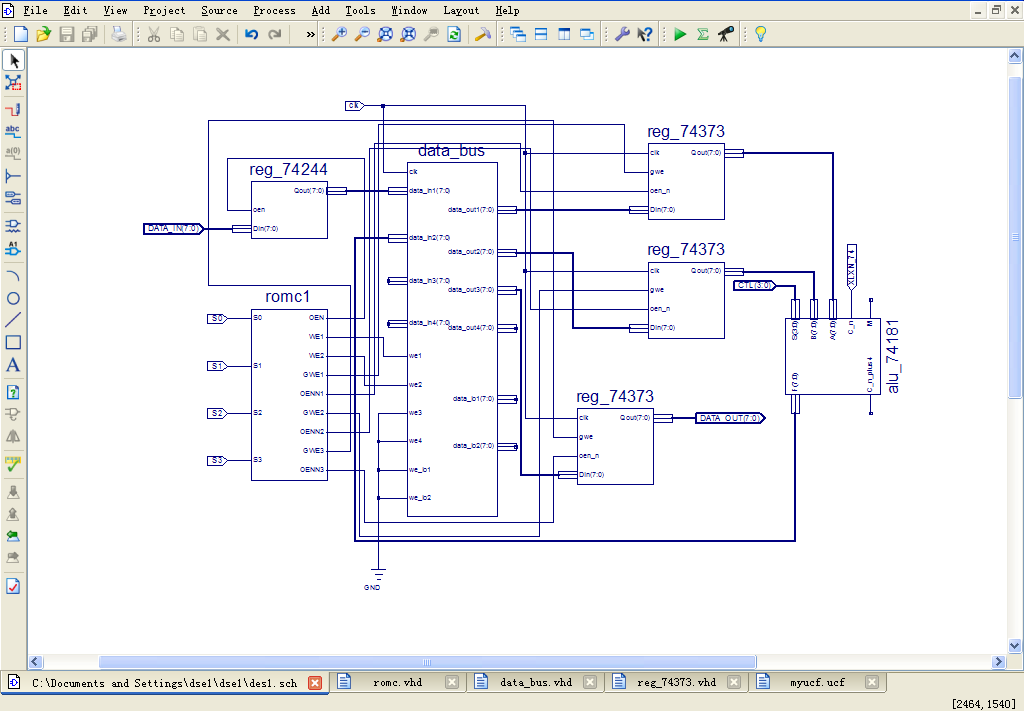
\includegraphics[width=\textwidth]{figure/final.PNG}
	\caption{ISE中的元件线路图}\label{fig:线路图}
\end{figure}

\subsection{简单加法器测试}
将元件线路图中的romc元件定义修改为附录\ref{简单加法器romc程序}中的元件定义,对工程进行编译并下载到Xilink测试平台,保持CTL(3:0)(EES261的开关SW5$\sim$SW8)为0110,按照\ref{简单加法器指令结构}节中给出的指令执行顺序改变微指令输入S0/1/2/3(拨动Atlys开发板上的开关sw0/1/2/3),在输入端DATA\_IN(7:0)(EES261的开关SW9$\sim$SW16)输入两个数相加,观察输出结果DATA\_OUT(7:0)(EES261的LED灯LED1$\sim$LED8)。

\subsection{循环加法器测试}
将元件线路图中的romc元件定义修改为附录\ref{循环加法器romc程序}中的元件定义,对工程进行编译并下载到Xilink测试平台,保持CTL(3:0)为0110,按照\ref{循环加法器指令结构}节中给出的指令执行顺序改变微指令输入S0/1/2/3,在输入端DATA\_IN(7:0)输入多个数相加,观察每一步的输出结果DATA\_OUT(7:0)。

\subsection{测试结果}
\subsubsection{简单加法器运行测试结果}
当DATA\_IN输入的两个数为00000001时,DATA\_OUT输出为00000010,表明简单加法器CPU能正常工作。

\subsubsection{循环加法器运行测试结果}
当DATA\_IN输入保持为00000001时,DATA\_OUT在每次循环中都会加一,表明循环加法器CPU能正常工作。

\section{总结}
\subsection{遇到的问题}
本次设计中遇到的主要问题是romc的VHDL程序输出位的顺序问题,开始测试时在romc的VHDL程序中将微指令译码得到的romc控制位输出写反导致测试结果不正确,错误排查花费了较多时间。

此外,本次设计中还遇到了循环运算的问题。由于输入指令的方式为手拨开关,因此每个命令之间都会经过多个时钟周期,若此时romc的WE2和GWE1(或GWE2)同时输出高电平,则总线会循环进行“从输入寄存器中取出一个数放入数据寄存器1(或2)中$\rightarrow$从算术逻辑单元中取出运算结果放入数据寄存器1(或2)中”,导致数据寄存器内的值不断自增,使得输出结果不正确,错误排查花费了一定时间。

\subsection{心得体会}
\begin{itemize}
	\item 更加深入地理解了计算机CPU的工作原理;
	\item 对计算机的体系结构有了更加深入的了解;
	\item 巩固了计算机组成原理的知识;
	\item 初步掌握了VHDL语言和ISE的使用方法。
\end{itemize}

\end{spacing}
\newpage
\section*{附录}\addcontentsline{toc}{section}{附录}\appendix
\section{alu\_74181修改后的VHDL程序}\label{alu_74181程序}
\begin{lstlisting}
library IEEE;
use IEEE.STD_LOGIC_1164.ALL;
use IEEE.STD_LOGIC_ARITH.ALL;
use IEEE.STD_LOGIC_UNSIGNED.ALL;

use IEEE.NUMERIC_STD.ALL;

entity alu_74181 is
	Port ( A : in  STD_LOGIC_VECTOR (7 downto 0);
			B : in  STD_LOGIC_VECTOR (7 downto 0);
			S : in  STD_LOGIC_VECTOR (3 downto 0);
			M : in  STD_LOGIC;
			C_n : in  STD_LOGIC;
			F : out  STD_LOGIC_VECTOR (7 downto 0);
			C_n_plus4 : out  STD_LOGIC);
end alu_74181;

architecture Behavioral of alu_74181 is

signal data_o_logic : STD_LOGIC_VECTOR (7 downto 0);
signal data_o_arith : STD_LOGIC_VECTOR (8 downto 0);

signal data_sub_tmp : STD_LOGIC_VECTOR (8 downto 0);

signal C_n_arith : STD_LOGIC_VECTOR (8 downto 0);

begin

	F <= data_o_logic when M = '1' else
			data_o_arith(7 downto 0);
	-- carry out	  
	C_n_plus4 <= not data_o_arith(4) when M = '0' else '1';
	
	C_n_arith <= "00000000" & (not C_n);

	-- 74181 logic operation
	process(A,B,S,M)
	begin
		case (S) is 
			when "0000" =>
				data_o_logic <= not A;
			when "0001" =>
				data_o_logic <= not (A or B);
			when "0010" =>
				data_o_logic <= (not A) and B;
			when "0011" =>
				data_o_logic <= (others => '0');
			when "0100" =>
				data_o_logic <= not (A and B);
			when "0101" =>
				data_o_logic <= not B;
			when "0110" =>
				data_o_logic <= (A xor B);
			when "0111" =>
				data_o_logic <= A and (not B);
			when "1000" =>
				data_o_logic <= (not A) or B;
			when "1001" =>
				data_o_logic <= (A xnor B);
			when "1010" =>
				data_o_logic <= B;
			when "1011" =>
				data_o_logic <= A and B;
			when "1100" =>
				data_o_logic <= "00000001";
			when "1101" =>
				data_o_logic <= A or (not B);
			when "1110" =>
				data_o_logic <= A or B;
			when "1111" =>
				data_o_logic <= A;
			when others =>
				data_o_logic <= (others => '0');
		end case;
	end process;

	-- 74181 arithmetic operation
	process(A,B,S,M,C_n_arith)
	begin
		case (S) is 
			when "0000" =>
				data_o_arith <= ('0'&A) + C_n_arith;
			when "0001" =>
				data_o_arith <= '0'&(A or B) + C_n_arith;
			when "0010" =>
				data_o_arith <= '0'&(A or (not B)) + C_n_arith;
			when "0011" =>
				-- if C_n = 0, minus 1,carry bit is 0; if C_n = 1,carry bit is 1;
				data_o_arith <= "01111" + C_n_arith; 
			when "0100" =>
				data_o_arith <= ('0'&A) + ('0'&(A and (not B))) + C_n_arith;
			when "0101" =>
				data_o_arith <= ('0'&(A or B))+('0'&(A and (not B)))+ C_n_arith;
			when "0110" =>
				-- if sub function, carry bit is different from add function
				data_sub_tmp <= ('0'&A) - ('0'&B) - 1 + C_n_arith;
				data_o_arith <= not data_sub_tmp(4) & data_sub_tmp(7 downto 0);
			when "0111" =>
				-- if sub function, carry bit is different from add function
				data_sub_tmp <= ('0'&(A and (not B)))- 1 + C_n_arith;
				data_o_arith <= not data_sub_tmp(4) & data_sub_tmp(7 downto 0);
			when "1000" =>
				data_o_arith <= ('0'&A) +('0'&(A and B))+ C_n_arith;
			when "1001" =>
				data_o_arith <= ('0'&A) + ('0'&B) + C_n_arith;
			when "1010" =>
				data_o_arith <= ('0'&(A or (not B))) + ('0'&(A and B))+ C_n_arith;
			when "1011" =>
				-- if sub function, carry bit is different from add function
				data_sub_tmp <= ('0'&(A and B)) - 1 + C_n_arith;
				data_o_arith <= not data_sub_tmp(4) & data_sub_tmp(7 downto 0);
			when "1100" =>
				data_o_arith <= ('0'&A) + ('0'&A) + C_n_arith;
			when "1101" =>
				data_o_arith <= ('0'&(A or B)) + ('0'&A) + C_n_arith;
			when "1110" =>
				data_o_arith <= ('0'&(A or (not B))) + ('0'&A) + C_n_arith;
			when "1111" =>
				-- if sub function, carry bit is different from add function
				data_sub_tmp <= ('0'&A) - 1 + C_n_arith;
				data_o_arith <= not data_sub_tmp(4) & data_sub_tmp(7 downto 0);
		
			when others =>
				data_o_arith <= (others => '0');
		end case;
	end process;
end Behavioral;	
\end{lstlisting}

\newpage
\section{简单加法器romc修改后的VHDL程序}\label{简单加法器romc程序}
\begin{lstlisting}
library IEEE;
use IEEE.STD_LOGIC_1164.ALL;

entity romc1 is
	Port ( S0 : in  STD_LOGIC;
			S1 : in  STD_LOGIC;
			S2 : in  STD_LOGIC;
			S3 : in  STD_LOGIC;
			OEN : out  STD_LOGIC;
			WE1 : out  STD_LOGIC;
			WE2 : out  STD_LOGIC;
			GWE1 : out  STD_LOGIC;
			OENN1 : out  STD_LOGIC;
			GWE2 : out  STD_LOGIC;
			OENN2 : out  STD_LOGIC;
			GWE3 : out  STD_LOGIC;
			OENN3 : out  STD_LOGIC);
end romc1;

architecture Behavioral of romc1 is
	signal addr  : std_logic_vector(3 downto 0);  --input
	signal rdata : std_logic_vector(8 downto 0);  --output
begin

addr <= s3 & s2 & s1 & s0 ;
	process(addr)
		begin
		case (addr) is
			when "0000" => rdata <= "101011010";
			when "0001" => rdata <= "101110010";
			when "0011" => rdata <= "010000100";
			when others => rdata <= "000000000";
		end case;
	end process;
		
	OEN<=rdata(0);
	WE1<=rdata(1);
	WE2<=rdata(2);
	GWE1<=rdata(3);
	OENN1<=rdata(4);
	GWE2<=rdata(5);
	OENN2<=rdata(6);
	GWE3<=rdata(7);
	OENN3<=rdata(8);
end Behavioral;	
\end{lstlisting}

\newpage
\section{循环加法器romc修改后的VHDL程序}\label{循环加法器romc程序}
\begin{lstlisting}
library IEEE;
use IEEE.STD_LOGIC_1164.ALL;

entity romc1 is
    Port ( S0 : in  STD_LOGIC;
           S1 : in  STD_LOGIC;
           S2 : in  STD_LOGIC;
           S3 : in  STD_LOGIC;
           OEN : out  STD_LOGIC;
           WE1 : out  STD_LOGIC;
           WE2 : out  STD_LOGIC;
           GWE1 : out  STD_LOGIC;
           OENN1 : out  STD_LOGIC;
           GWE2 : out  STD_LOGIC;
           OENN2 : out  STD_LOGIC;
           GWE3 : out  STD_LOGIC;
           OENN3 : out  STD_LOGIC);
end romc1;

architecture Behavioral of romc1 is
    signal addr  : std_logic_vector(3 downto 0);  --input
    signal rdata : std_logic_vector(8 downto 0);  --output
begin

addr <= s3 & s2 & s1 & s0 ;
	
    process(addr)
	 begin
		case (addr) is
			when "0000" => rdata <= "101010010";
			when "0001" => rdata <= "101011000";
			when "0010" => rdata <= "101110000";
			when "0011" => rdata <= "010000100";
			when "0111" => rdata <= "101110000";
			when "1111" => rdata <= "101011010";
			when "1110" => rdata <= "010000100";
			when "1100" => rdata <= "101110000";
			when "1000" => rdata <= "101011010";
			when "1001" => rdata <= "010000100";
			when "1011" => rdata <= "101110000";
			when others => rdata <= "000000000";
		end case;
	end process;
	 
	OEN<=rdata(0);
    WE1<=rdata(1);
    WE2<=rdata(2);
    GWE1<=rdata(3);
    OENN1<=rdata(4);
    GWE2<=rdata(5);
    OENN2<=rdata(6);
    GWE3<=rdata(7);
    OENN3<=rdata(8);
end Behavioral;
\end{lstlisting}

\newpage
\section{外部端口定义}\label{外部端口定义}
\begin{lstlisting}
###------------CLOCK-----------
NET "clk"   LOC = "L15";
#
###-----------Atlys Switch input-------------------
NET "S0"    LOC = A10;  # Atlys sw0
NET "S1"    LOC = D14;  # Atlys sw1
NET "S2"    LOC = C14;  # Atlys sw2
NET "S3"    LOC = P15;  # Atlys sw3
#NET "atlys_sw[4]"    LOC = P12;  # Atlys sw4
#NET "atlys_sw[5]"    LOC = R5;   # Atlys sw5
#NET "atlys_sw[6]"    LOC = T5;   # Atlys sw6
NET "XLXN_74"    LOC = E4;   # Atlys sw7
#
###------------EES261 switch input----------
#NET "swt[19]" LOC = "U11";    #SW20
#NET "swt[18]" LOC = "R10";    #SW19
#NET "swt[17]" LOC = "U10";   #SW18
#NET "swt[16]" LOC = "R8";   #SW17
#
NET "DATA_IN[7]" LOC = "M8";  #SW16
NET "DATA_IN[6]" LOC = "U8";   #SW15
NET "DATA_IN[5]" LOC = "U7";   #SW14
NET "DATA_IN[4]" LOC = "N7";   #SW13
#
NET "DATA_IN[3]" LOC = "T6";   #SW12
NET "DATA_IN[2]" LOC = "R7";   #SW11
NET "DATA_IN[1]" LOC = "N6";    #SW10
NET "DATA_IN[0]" LOC = "U5";    #SW9
#
NET "CTL[3]" LOC = "V5";    #SW8
NET "CTL[2]" LOC = "P7";    #SW7
NET "CTL[1]" LOC = "T7";    #SW6
NET "CTL[0]" LOC = "V6";    #SW5
#
##----------EES261  leds output------------
NET "DATA_OUT<0>" LOC = "U16";    #LED1
NET "DATA_OUT<1>" LOC = "U15";    #LED2
NET "DATA_OUT<2>" LOC = "U13";    #LED3
NET "DATA_OUT<3>" LOC = "M11";    #LED4
NET "DATA_OUT<4>" LOC = "R11";    #LED5
NET "DATA_OUT<5>" LOC = "T12";    #LED6
NET "DATA_OUT<6>" LOC = "N10";    #LED7
NET "DATA_OUT<7>" LOC = "M10";    #LED8
#
\end{lstlisting}
\end{document}